\lecture

\begin{guiding}
Two tasks. First, ground the Euler class in examples: canonical bundles over
projective lines, and the universal identity $e(\gamma^n)=\tilde\sigma_n$.
Second, pay the outstanding debt and prove the Thom isomorphism theorem.
\end{guiding}

\section{Euler classes of canonical bundles}

\begin{example}[The M\"obius band]\label{ex:mobius-euler}
Consider $\RP^1\hookrightarrow\RP^2$, $[x_0,x_1]\mapsto[x_0,x_1,0]$. The
complement of $\RP^1$ is the affine chart $\{x_2\neq0\}\iso\R^2$, an open disc,
and a neighbourhood of $\RP^1$ in $\RP^2$ is the total space of its normal
bundle, which is $\gamma^1_1$. Hence
\[
\RP^2=\big(\text{M\"obius band}\big)\cup_{\partial}D^2 .
\]

\begin{center}
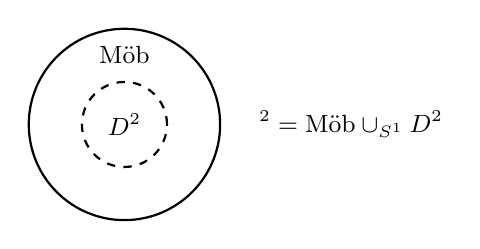
\begin{tikzpicture}[scale=0.9]
\draw[thick] (0,0) circle (1.35);
\draw[thick,dashed] (0,0) circle (0.6);
\node at (0,0) {\small $D^2$};
\node at (0,0.98) {\small M\"ob};
\node at (3.2,0) {\small $\RP^2=\mathrm{M\ddot ob}\cup_{S^1}D^2$};
\end{tikzpicture}
\end{center}

The pair $(E,E_0)$ for $\gamma^1_1$ deformation retracts onto (M\"obius band,
boundary), so with $\Z_2$ coefficients
\[
H^{*>0}\big(\gamma^1_1,(\gamma^1_1)_0\big)
\iso H^{*>0}\big(\RP^2\big)=\Z_2[a]/(a^3),
\]
by excising the complementary disc. Under this identification the Thom class $u$
corresponds to $a$, so $u\smile u$ corresponds to $a^2\neq0$. This is the
computation quoted in Step 4 of the previous lecture, and it gives
$w_1(\gamma^1_1)\neq0$ once more, now by Thom-theoretic means.
\end{example}

\begin{example}[The complex canonical bundle]\label{ex:e-gamma-CP1}
Let $\gamma_1\to\CP^1$ be the tautological complex line bundle. Exactly as above,
$\CP^1\subset\CP^2$ has normal bundle $\gamma_1$ and complementary affine chart
a $4$-disc, so
\[
\CP^2=E\big(\gamma_1\big)\cup_{S^3}D^4 ,
\]
and $H^*(E,E_0;\Z)\iso H^{*>0}(\CP^2;\Z)$, generated by $u$ in degree $2$ with
$u^2$ generating degree $4$. Chasing $u$ through
$H^2(E,E_0)\to H^2(E)\iso H^2(\CP^1)$ identifies
\[
e\big(\gamma_1\to\CP^1\big)=a,
\]
a generator of $H^2(\CP^1;\Z)$. Note that every complex bundle is canonically
oriented, by declaring $v_1,Jv_1,\dots,v_n,Jv_n$ positive for any complex basis
$v_1,\dots,v_n$; so the Euler class of a complex bundle is defined without extra
choices.
\end{example}

\begin{theorem}\label{thm:e-gamma-n}
$e(\gamma_n)=\tilde\sigma_n=c_n(\gamma_n)$ for the universal complex bundle,
and over $\Z_2$, $e(\gamma^n)=\tilde\sigma_n=w_n(\gamma^n)$ for the universal
real bundle. Consequently, for every bundle $\xi$,
\[
e(\xi)=c_n(\xi)\ \ (\xi \text{ complex}),
\qquad
e(\xi)\bmod2=w_n(\xi)\ \ (\xi \text{ real oriented}).
\]
\end{theorem}

\begin{proof}
\begin{strategy}
Compute the Euler class of a sum of $n$ line bundles over $(\CP^\infty)^n$,
where multiplicativity turns it into $a_1\cdots a_n=\sigma_n$; then use that
$h_n^*$ is injective to transport the identity to the universal bundle.
\end{strategy}

\step{1} \emph{Stabilizing.} The inclusion $\CP^1\hookrightarrow\CP^\infty$ is
covered by a bundle map $\gamma_1\to\gamma_1$ and induces an isomorphism on
$H^2$. By naturality and Example~\ref{ex:e-gamma-CP1},
$e(\gamma_1\to\CP^\infty)=a$, the generator of $H^2(\CP^\infty;\Z)=\Z[a]$.

\step{2} \emph{Sums of lines.} Over $(\CP^\infty)^n$, by
Theorem~\ref{thm:euler-properties}(5),
\[
e\big(\gamma_1\oplus\dots\oplus\gamma_1\big)
=e(\gamma_1)\smile\dots\smile e(\gamma_1)
=a_1a_2\cdots a_n=\sigma_n(a_1,\dots,a_n).
\]

\step{3} \emph{Transport.} Let $h_n\colon(\CP^\infty)^n\to G_n(\C^\infty)$
classify that sum, so $h_n^*\gamma_n\iso\gamma_1\oplus\dots\oplus\gamma_1$. By
naturality of the Euler class,
$h_n^*e(\gamma_n)=\sigma_n=h_n^*(\tilde\sigma_n)$, and $h_n^*$ is injective by
Theorem~\ref{thm:HGnC}; hence $e(\gamma_n)=\tilde\sigma_n=c_n(\gamma_n)$.

\step{4} \emph{Real case and general bundles.} The same three steps over
$\RP^\infty$ with $\Z_2$ coefficients give $e(\gamma^n)=\tilde\sigma_n$. For an
arbitrary bundle, pull back along a classifying map and use naturality of both
$e$ and the characteristic classes.
\end{proof}

\section{Proof of the Thom isomorphism theorem}

We now prove Theorem~\ref{thm:thom}. Throughout, $\pi\colon E\to B$ has rank $n$
and $E_0$ is the complement of the zero section. The model computation is the
following consequence of K\"unneth.

\begin{lemma}\label{lem:suspension}
Let $e^1\in H^1(\R,\R_0;\Lambda)$ be a generator, where $\R_0=\R\smallsetminus0$
and $\Lambda$ is any coefficient ring. Then for every space $B$ and every open
$B'\subset B$ the map
\[
H^{j}(B,B')\longrightarrow
H^{j+1}\big(B\times\R,\ B'\times\R\cup B\times\R_0\big),
\qquad
y\longmapsto y\times e^1,
\]
is an isomorphism; iterating $n$ times, with $e^n=e^1\times\dots\times e^1$,
\[
H^{j}(B,B')\ \xrightarrow{\ \cong\ }\
H^{j+n}\big(B\times\R^n,\ B'\times\R^n\cup B\times\R^n_0\big),
\qquad y\longmapsto y\times e^n .
\]
\end{lemma}

\begin{proof}
The pair $(\R,\R_0)$ has cohomology $\Lambda$ concentrated in degree $1$,
generated by $e^1$, and it is free; the relative K\"unneth theorem therefore
gives
\[
H^{j+1}\big(B\times\R,\ B'\times\R\cup B\times\R_0\big)
\iso\bigoplus_{p+q=j+1}H^p(B,B')\otimes H^q(\R,\R_0)
=H^{j}(B,B')\otimes\Lambda ,
\]
and the isomorphism is exactly $y\mapsto y\times e^1$. Iterate.
\end{proof}

\begin{proof}[Proof of Theorem~\ref{thm:thom}]
\begin{strategy}
Four stages of increasing generality. For a trivial bundle the statement is
Lemma~\ref{lem:suspension}. If the base splits into two open pieces over which
the theorem is known, Mayer--Vietoris and the five lemma give it over the union;
a finite trivializing cover then handles compact bases. Arbitrary bases follow
by writing cohomology as a limit over compact subsets, which works with field
coefficients. Finally an algebraic lemma about mapping cones upgrades field
coefficients to $\Z$.
\end{strategy}

\step{1} \emph{Case 1: $E$ trivial.} Here
$(E,E_0)\iso(B\times\R^n,B\times\R^n_0)$. Taking $B'=\emptyset$ in
Lemma~\ref{lem:suspension} gives
\[
H^j(B)\ \iso\ H^{j+n}(E,E_0),\qquad y\mapsto y\times e^n .
\]
In particular $H^{j+n}(E,E_0)=0$ for $j<0$, and $H^n(E,E_0)\iso H^0(B)$. Put
$u=1\times e^n$. Its restriction to a fibre pair is $e^n$, the preferred
generator, so $u$ is a Thom class; and it is unique because a class restricting
to $0$ on every fibre corresponds to $y\times e^n$ with $y$ vanishing at every
point of $B$, hence $y=0$. Finally, elements of $H^j(E)=H^j(B\times\R^n)$ are of
the form $y\times1$, and
\[
(y\times1)\smile u=(y\times1)\smile(1\times e^n)=y\times e^n,
\]
so $\smile u$ is the isomorphism just described.

\step{2} \emph{Case 2: Mayer--Vietoris.} Suppose $B=B'\cup B''$ with $B',B''$
open and the theorem known over $B'$, $B''$ and $B^\cap=B'\cap B''$. Write
$E',E'',E^\cap$ for the restrictions of $E$. Consider the Mayer--Vietoris
sequence of the pairs,
\[
H^{n-1}(E^\cap,E_0^\cap)\longrightarrow H^n(E,E_0)
\xrightarrow{\ (i'^*,\,i''^*)\ }H^n(E',E'_0)\oplus H^n(E'',E''_0)
\]
\[
\xrightarrow{\ i'^*-i''^*\ }H^n(E^\cap,E^\cap_0).
\]
By hypothesis $H^{n-1}(E^\cap,E^\cap_0)\iso H^{-1}(B^\cap)=0$. The classes
$u',u''$ both restrict to the unique Thom class $u^\cap$ of $E^\cap$, so the
pair $(u',u'')$ dies under $i'^*-i''^*$ and lifts to a unique
$u\in H^n(E,E_0)$; it restricts to the preferred generator on every fibre, since
every fibre lies over $B'$ or $B''$. Now $\smile u$ maps the Mayer--Vietoris
sequence of $(B',B'')$ to that of $(E',E'')$, commutatively; the maps over
$B',B'',B^\cap$ are isomorphisms by hypothesis, so the five lemma gives the
result over $B$.

\step{3} \emph{Case 3: $B$ compact.} Choose a finite trivializing cover
$U_1,\dots,U_r$. By Case 1 the theorem holds over each $U_i$ and over each
intersection, which is again trivializing. By Case 2 it holds over
$U_1\cup U_2$; inductively, if it holds over $U_1\cup\dots\cup U_j$ then apply
Case 2 to that set together with $U_{j+1}$, whose intersection with it is a
union of $j$ trivializing sets covered by the inductive hypothesis. After $r$
steps we reach $B$.

\step{4} \emph{Case 4: general base, field coefficients.} Every singular chain
has compact image, so
$H_j(B)=\varinjlim_C H_j(C)$ over the compact subsets $C\subset B$. With
\emph{field} coefficients $\Lambda$, cohomology is the dual of homology, and
duals turn direct limits into inverse limits:
\[
H^j(B;\Lambda)=\Hom\big(\varinjlim_C H_j(C),\Lambda\big)
=\varprojlim_C\Hom\big(H_j(C),\Lambda\big)=\varprojlim_C H^j(C;\Lambda),
\]
and similarly for the pairs $(E,E_0)$ restricted over $C$. By Case 3 there is a
compatible Thom class over each $C$, and compatible isomorphisms; passing to the
inverse limit gives a Thom class $u$ over $B$, its uniqueness, and the
isomorphism $\smile u$. This already proves the theorem over $\Z_2$ for
arbitrary bundles, which is all that Stiefel--Whitney theory requires.

\step{5} \emph{Integral coefficients.} Two further ingredients are needed, and
they occupy the rest of the lecture: the algebraic Lemma~\ref{lem:alg} below,
and the vanishing $H_{n-1}(E,E_0;\Z)=0$. Granting the latter, universal
coefficients,
\[
0\to\Ext\big(H_{n-1}(E,E_0),\Z\big)\to H^n(E,E_0;\Z)\to
\Hom\big(H_n(E,E_0),\Z\big)\to0,
\]
gives $H^n(E,E_0;\Z)\iso\Hom(H_n(E,E_0),\Z)$, and the compatible fibrewise
normalization determines a unique integral $u$. Choose a singular cocycle
$z\in Z^n(E,E_0)$ representing $u$. Cap product with $z$ is a chain map of
degree $-n$,
\[
z\,\cap\ \colon\ C_{n+i}(E,E_0)\longrightarrow C_i(E),
\qquad
\partial(z\cap\gamma)=(-1)^n z\cap\partial\gamma,
\]
whose dual on cochains is $c\mapsto c\smile z$. By Step 4 the induced map on
cohomology is an isomorphism over every field. By Lemma~\ref{lem:alg} it is then
an isomorphism over $\Z$, and over any coefficient ring.
\end{proof}

\begin{lemma}\label{lem:alg}
Let $f\colon K\to K'$ be a chain map of free chain complexes over $\Z$ which
induces isomorphisms $H^*(K';\Lambda)\to H^*(K;\Lambda)$ for every field
$\Lambda$. Then $f$ induces isomorphisms on homology and cohomology with any
coefficient ring.
\end{lemma}

\begin{proof}
\begin{strategy}
Encode ``$f$ is a homology isomorphism'' as the vanishing of the homology of the
algebraic mapping cone. That homology is finitely constrained by universal
coefficients: rational coefficients show it is torsion, and $\Z_p$ coefficients
show it has no $p$-torsion for any prime $p$.
\end{strategy}

\step{1} \emph{The mapping cone.} Let $d$ be the degree of $f$ and put
$K^f_i=K_{i-d-1}\oplus K'_i$ with
\[
\partial^f(k,k')=\big((-1)^{d+1}\partial k,\ f(k)+\partial k'\big).
\]
A direct computation gives $\partial^f\circ\partial^f=0$, using
$\partial f=(-1)^d f\partial$. The complex $K^f$ is free.

\step{2} \emph{The long exact sequence.} There is a short exact sequence of
complexes $0\to K'\to K^f\to K[\,d+1\,]\to0$, whose long exact sequence has
connecting homomorphism induced by $f$:
\[
\cdots\to H_i(K')\to H_i(K^f)\to H_{i-d-1}(K)
\xrightarrow{\ f_*\ }H_{i-1}(K')\to\cdots
\]
Hence $H_*(K^f)=0$ if and only if $f_*$ is an isomorphism on homology.

\step{3} \emph{Vanishing over every field.} By hypothesis $f$ induces
isomorphisms on cohomology with field coefficients, so the corresponding
sequence gives $H^*(K^f;\Lambda)=0$ for every field $\Lambda$. Universal
coefficients,
\[
0\to\Ext\big(H_{q-1}(K^f),\Lambda\big)\to H^q(K^f;\Lambda)\to
\Hom\big(H_q(K^f),\Lambda\big)\to0,
\]
then forces $\Hom(H_q(K^f),\Lambda)=0$ for every field.

\step{4} \emph{Conclusion.} Taking $\Lambda=\Q$ shows $H_q(K^f)$ has no free
part, so it is a torsion group. Taking $\Lambda=\Z_p$ and using also the $\Ext$
term shows $H_q(K^f)$ has no $p$-torsion, for every prime $p$. Hence
$H_q(K^f)=0$ for all $q$, and by Step 2 the map $f$ is a homology isomorphism
over $\Z$; the same then holds with any coefficients, again by universal
coefficients applied to the free complexes.
\end{proof}

\begin{corollary}\label{cor:cap-thom}
For an oriented rank $n$ bundle, the cap product with the Thom class,
\[
H_{n+i}(E,E_0;\Lambda)\longrightarrow H_i(E;\Lambda),
\qquad
\eta\longmapsto u\cap\eta,
\]
is an isomorphism for every coefficient ring $\Lambda$, compatibly with the
cohomological Thom isomorphism through
$\langle c,u\cap\gamma\rangle=\langle c\smile u,\gamma\rangle$.
\end{corollary}

\begin{remark}
It remains to justify $H_{n-1}(E,E_0;\Z)=0$, used in Step 5. For compact $B$
this follows from Corollary~\ref{cor:cap-thom} in the already established cases,
which gives $H_{n-1}(E,E_0)\iso H_{-1}(E)=0$; for general $B$ write
$H_{n-1}(E,E_0;\Z)=\varinjlim_C H_{n-1}(E|_C,E_0|_C;\Z)=0$, since homology
commutes with direct limits.
\end{remark}

With the Thom isomorphism established, the next lecture brings it into contact
with geometry: tubular neighbourhoods, dual classes of submanifolds, and the
diagonal.
